\subsection{Genome Instrumentation}
\label{sec:genome-instrumentation}

This section first reviews hereditary stratigraphy as originally developed for inference over asexual populations then introduces gene- and species-level hereditary stratigraphy instrumentation strategies to apply it to sexual populations.

Subsequent discussion covers recombination and ``gene drive'' mechanisms employed for species-level instrumentation.
Calculations assess expected elevation of spurious overestimations of relatedness due to the gene drive mechanism.


% \begin{figure}
  \centering
  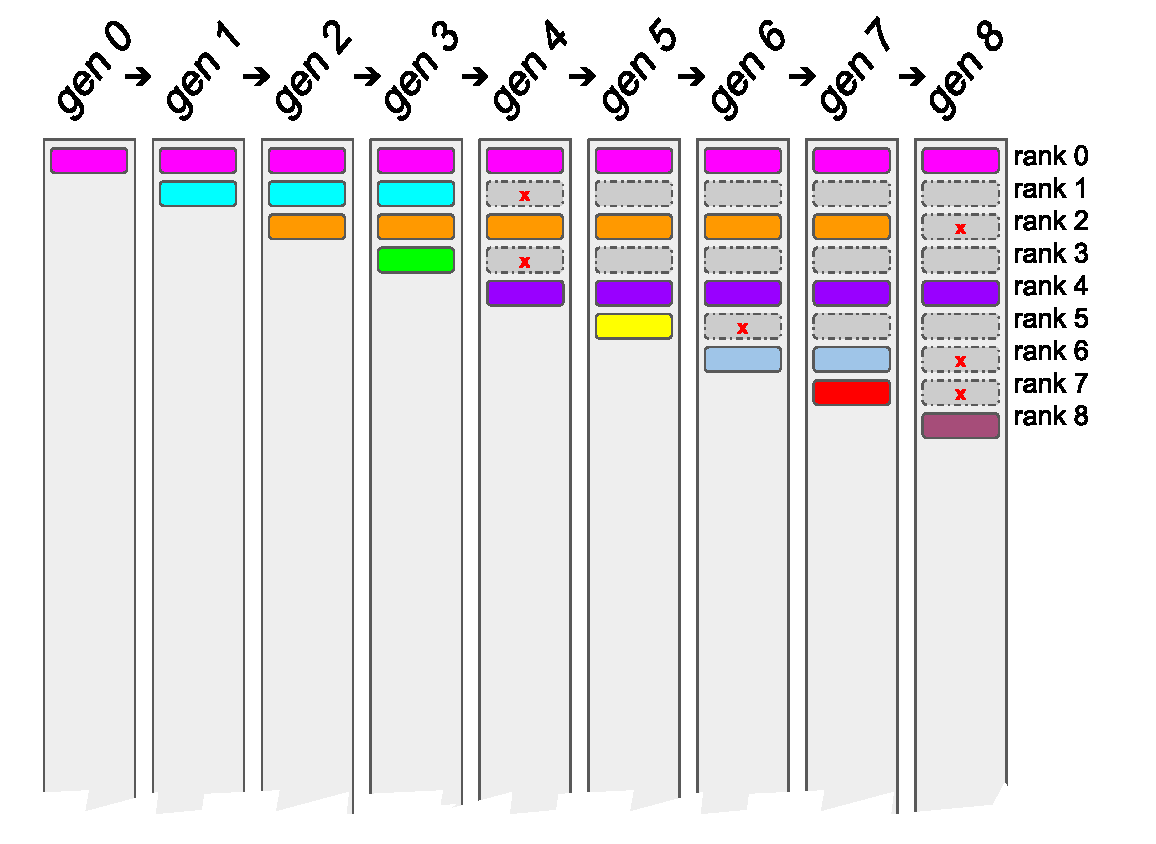
\includegraphics[width=\textwidth]{img/deposit-prune-example}
  \caption{
    TODO
  }
  \label{fig:deposit-prune-example}
\end{figure}

% \begin{figure}
  \centering
  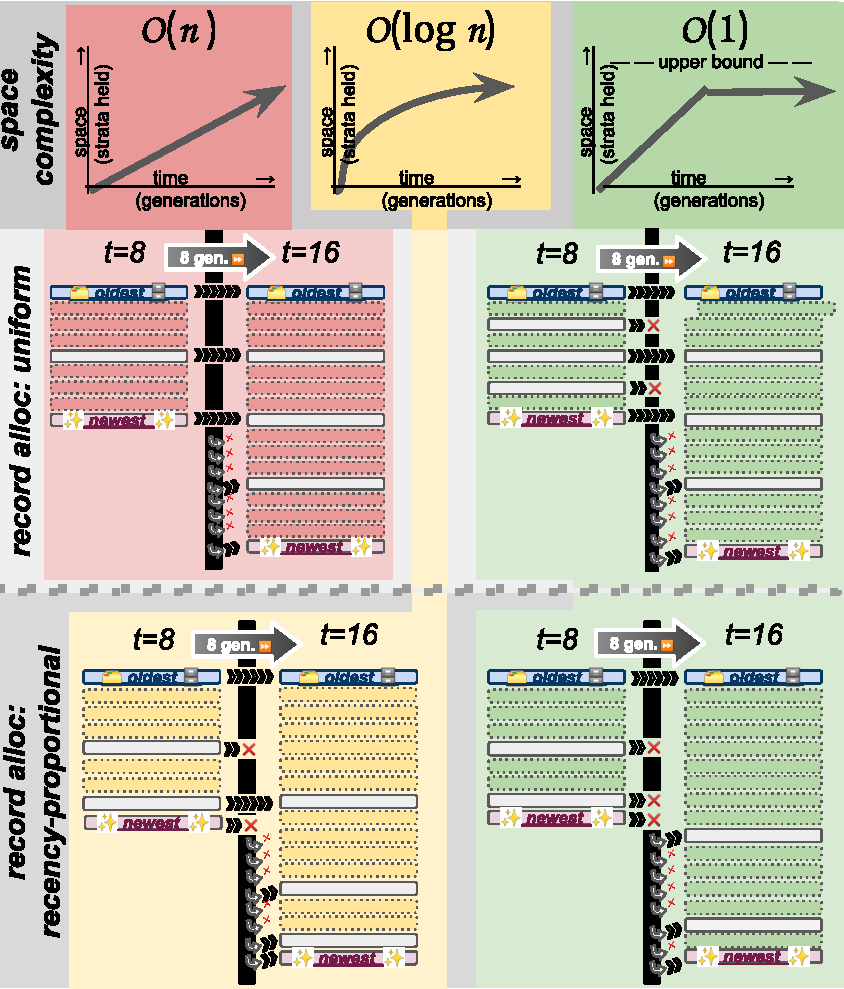
\includegraphics[width=\textwidth]{img/retention-policy-matrix}
  \caption{
    Comparison of four stratum retention policies by space complexity per stratigraph with respect to generations elapsed (columns, red/yellow/green) and by distribution of retained differentia (rows).
    Uniform allocation keeps differentia in evenly-spaced layers.
    Recency-proportional allocation keeps more more-recent differentia, trading off coarser resolution to infer ancient phylogenetic events for finer resolution to infer recent phylogenetic events.
    Retained layers under each policy are shown at $t=8$ generations and $t=16$ generations, with new differentia being deposited in a descending fashion.
    Differentia pruning events are noted with a red $x$.
  }
  \label{fig:retention-policy-matrix}
\end{figure}

\textbf{Hereditary Stratigraphy.}
Proposed methods for genealogical and evolutionary inference over distributed sexual populations draw on ``hereditary stratigraphy,'' originally developed to facilitate phylogenetic inference over asexual populations \citep{moreno2022hstrat}.
The core mechanism of this technique is generation-on-generation accumulation of randomized ``fingerprint'' packets.
Offspring inherit parents' fingerprint record and append an entry.
Then, this process repeats with the next generation.

Fingerprint values convey no function phenotypic information.
Rather, they should be considered simply as neutral ornamentation affixed to an underlying functional genome to instrument it.
Because they tag along with genomes across replication events, a system's phylogenetic history can be reconstructed by proxy based on
 hereditary stratigraph instruments.
Each accumulated fingerprint ultimately serves as a kind of linealogical checkpoint.
Because fingerprints are faithfully inherited each generation after their creation, discrepancy between coincident fingerprints held by two population members implies divergent ancestry at their shared time point.
So, last common ancestry necessarily precedes the first mismatching fingerprints.

Some attention must be paid to space complexity.
Proceeding naively, perpetual fingerprint accumulation with each generation would hopelessly bloat memory use.
Fortunately, the underlying inferential mechanism allows thinning out of fingerprints.
Pruned-away fingerprints introduce a commensurate uncertainty into estimation of two records' divergence generation.
If every other fingerprint was pruned, for example, divergence generations would only be estimable to within 2 generations.
In this way, configuration of what fingerprints to keep when directly administers the inherent trade-off between memory use and inferential power.
Although beyond present scope, significantly more can be said about this running fingerprint curation process.
For detail, refer to \citep{moreno2022hereditary}.

In order to simplify experimental setup and analysis, experiments reported here do not incorporate fingerprint pruning.
All inference mechanisms introduced here are, in principle, compatible with fingerprint pruning.
However, further work remains to directly investigate how pruning affects presented approaches' characterization of evolutionary history and dynamics.
Analogous work in asexual populations will provide some initial indications in this direction \citep{moreno2023toward}.

This work uses 64 bit fingerprints, which collide spuriously with negligible probability $2^{-64} \approx 5 \times 10^{-20}$.
At population size 100 over 200 generations, as in the first sets of reported experiments, the probability of any collision is miniscule, $< 2 \times 10^{-15}$.
At population size 200 over 400 generations, as in the last set of reported experiments, the probability of any collision is also miniscule, $< 5 \times 10^{-15}$.

\begin{SCfigure}[3][b]
  \centering
  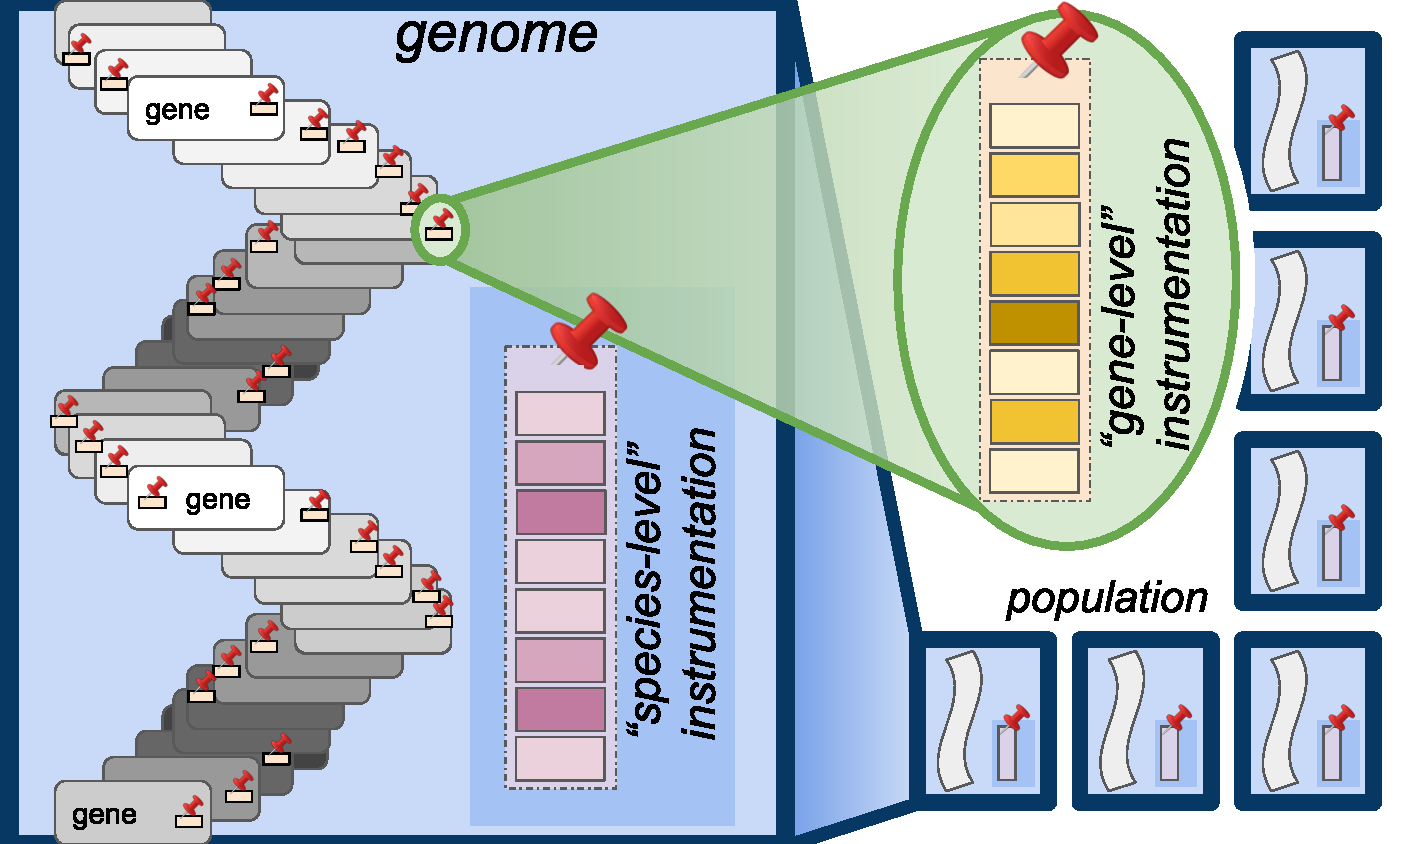
\includegraphics[width=0.5\textwidth]{img/annotation-types}
  \caption{
    Proposed instrumentation methods: ``species-level'' and ``gene-level'' instrumentation.
    Each organism has a single hereditary stratigraph attached as species-level instrumentation, with a gene drive mechanism (Figure \ref{fig:gene-drive}) ensuring consistentcy within species (i.e., interbreeding populations).
    Gene-level instrumentation associates instrumentation with individual genes, to be used for gene tree reconstructions.
  }
  \label{fig:annotation-types}
\end{SCfigure}

\textbf{Sexual Instrumentation Schemes.}
As originally devised for asexual populations, hereditary stratigraph annotations correspond one-to-one to genomes.
Here, we explore two alternate schemes designed for instrumentation of sexual populations: gene instrumentation and species instrumentation.
Figure \ref{fig:annotation-types} compares these two schemes.

Gene-level instrumentation treats individual genes simply as asexual atoms, instrumenting genes individually.
Reconstructions, therefore, fall along the lines of ``gene tree'' analsyes in traditional phylogenetics \citep{avise1989gene}.

In cases where genomes comprise relatively few genes, it may make sense to instrument every gene independently.
Other applications may warrant instrumenting only a subset of genes or introducing instrumented ``dummy'' genes.

Species-level instrumentation associates one instrument per genome.
Consensus within interbreeding populations arises through a ``gene drive'' mechanism (described below) that forces a single fingerprint value to sweep each fingerprint layer within species (i.e., interbreeding subpopulations).

Species-level instrumentation powers genealogical inference and population size inference (Sections \ref{sec:genealogical-inference} and \ref{sec:population-size-inference}).
Gene hereditary stratigraph instrumentation powers positive selection inference (Section \ref{sec:selection-inference}).

\begin{SCfigure}[3][b]
  \centering
  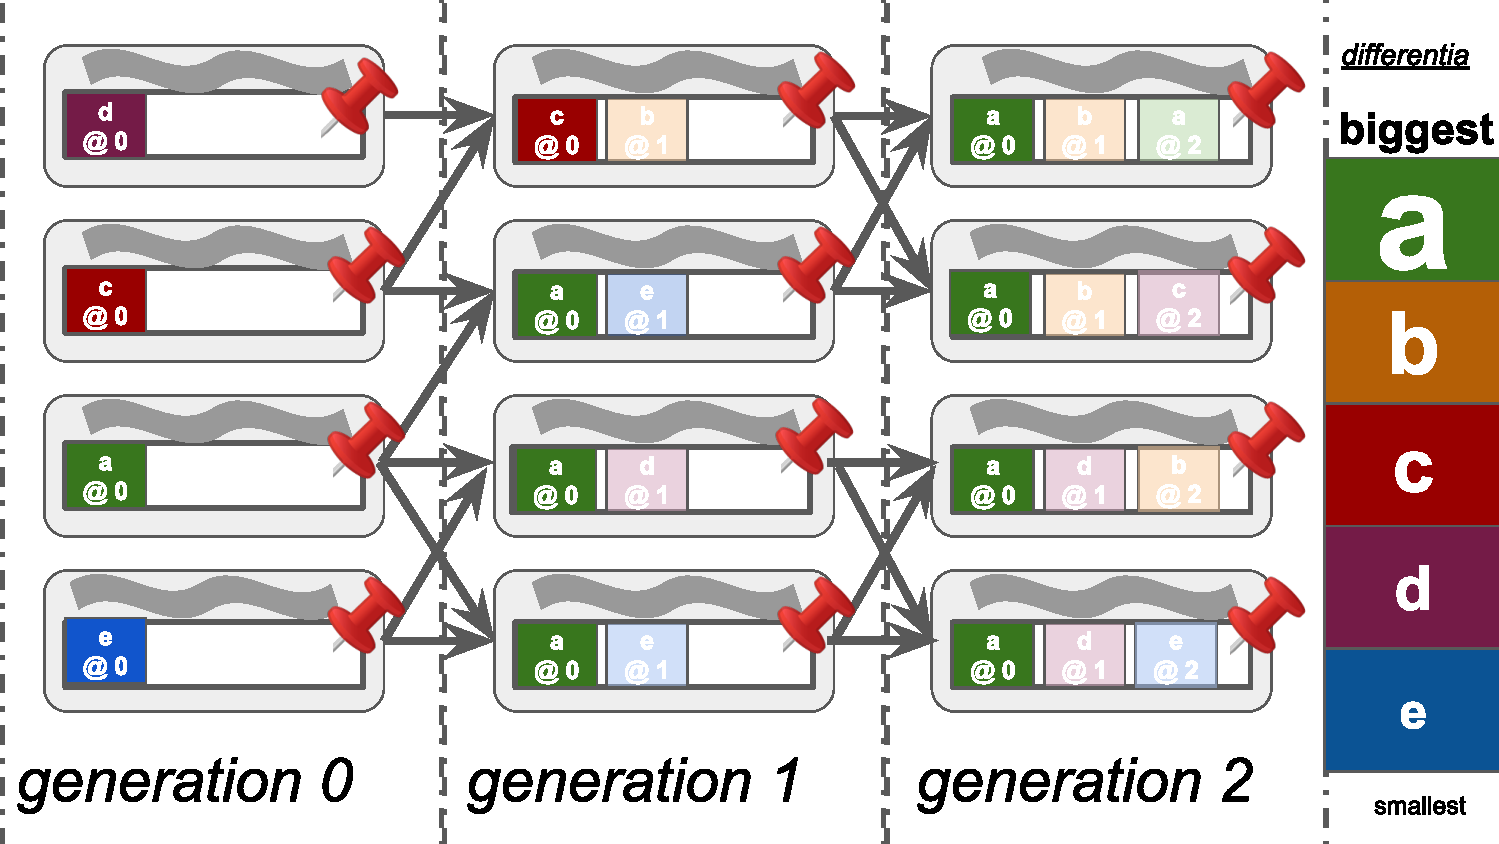
\includegraphics[width=0.6\textwidth]{img/gene-drive}
  \caption{
    Gene drive mechanism for species-level instrumentation.
    The larger of parents' differentia values at each layer is inherited.
    The largest value generated among layer 0 differentia ($a$) spreads from one member at generation 0 to all four by generation 2.
    This mechanism applies to ``species-level'' instrumentation (Figure \ref{fig:annotation-types}).
  }
  \label{fig:gene-drive}
\end{SCfigure}

\textbf{``Gene-drive'' Recombination Mechanism.}
Species-level tracking relies on consensus among corresponding-time-point fingerprint values within reproductively isolated subpopulations.
Under drift, such consensus would eventually arise.
However, time to coalescence through drift can be long for large populations
A simple inheritance rule reaches consensus faster: inherit the larger of parents' fingerpint values at each instrumentation layer.
Global maximum fingerprint values will spread rapidly and fix.
Figure \ref{fig:gene-drive} depicts this mechanism.

Asynchronous generations slightly complicate the picture.
When individuals from different generations recombine, one parent will have fingerprint layers absent in the other.
How should recombination proceed in this case?
One possibility would be to simply ``fast-forward'' the younger instrument to match the generational depth of the elder.
However, like with fingerprint pruning above, full consideration of asynchronous generations remains for future work.
All reported experiments use synchronous generations.

The gene-drive-based recombination mechanism described in this section applied exclusively to species-level instrumentation.
(Gene-level instruments, although tagging along with genes shuffled up through genome-level recombination, did not themselves recombine.)

\textbf{Fingerprint Collision Probability.}
Under gene-drive recombination, fixed fingerprints skew large due to the gene drive criterion.
This skew increases the probability of fingerprint collision between two populations causing spurious detection of shared ancestry.
This collision probability effect potentially threatens practicality of species-level instrumentaiton at scale.
We will assess the extent of this issue by computing threshold population sizes where collision becomes substantive.
Such calculations should be performed in applications of species-level instrumentation to choose appropriate sizes.

Suppose independent populations of size $a$ and $b$.
The largest fingerprint in each population will drive to fixation.
If each population members' gene is drawn from uniform distribution on integers $[0, u)$, then the probability of collision between the populations' fixed genes can be derived as

\begin{scriptsize}
\begin{align*}
\frac{a}{a + b}\sum_{n=1}^{a + b - 1} \frac{u^{- n - 1} \left(\frac{u - 1}{u}\right)^{a + b - n - 1} \left(1 - \frac{{\binom{a - 1}{n}}}{{\binom{a + b - 1}{n}}} \right) {\binom{a + b}{n + 1}}}{1 - \left(\frac{u - 1}{u}\right)^{a + b - 1}}
+ \frac{b}{a + b} \sum_{n=1}^{a + b - 1} \frac{u^{- n - 1} \left(\frac{u - 1}{u}\right)^{a + b - n - 1} \left(1 - \frac{{\binom{b - 1}{n}}}{{\binom{a + b - 1}{n}}} \right) {\binom{a + b}{n + 1}}}{1 - \left(\frac{u - 1}{u}\right)^{a + b - 1}}.
\end{align*}
\end{scriptsize}
% Derivation will be provided in supplementary materials. TODO?

For 32-bit differentia $u = 2^{32}$, collision occurs with $p < 0.5$ ($p = 0.46$) for populations of size $a = b = 2^{32}$.
Collision occurs with $p < 0.01$ for populations of size $a = b = 2^{26}$.
So, 32-bit fingerprints can differentiate species pairs of around $6.7 \times 10^{7}$ members each with reasonable consistency.%
\footnote{
Reported experiments used 64-bit fingerprint values, which will exhibit even lower collision probabilities.
However, numerical considerations complicate precise calculation.
}
